\definecolor{B128first}{HTML}{F6C928}
\definecolor{B256}{HTML}{36827F}
\definecolor{B128second}{HTML}{96A654}
\definecolor{B1024}{HTML}{464D77}

\begin{figure*}[t]
    \centering
    % \vspace{-0.6cm}
    %
    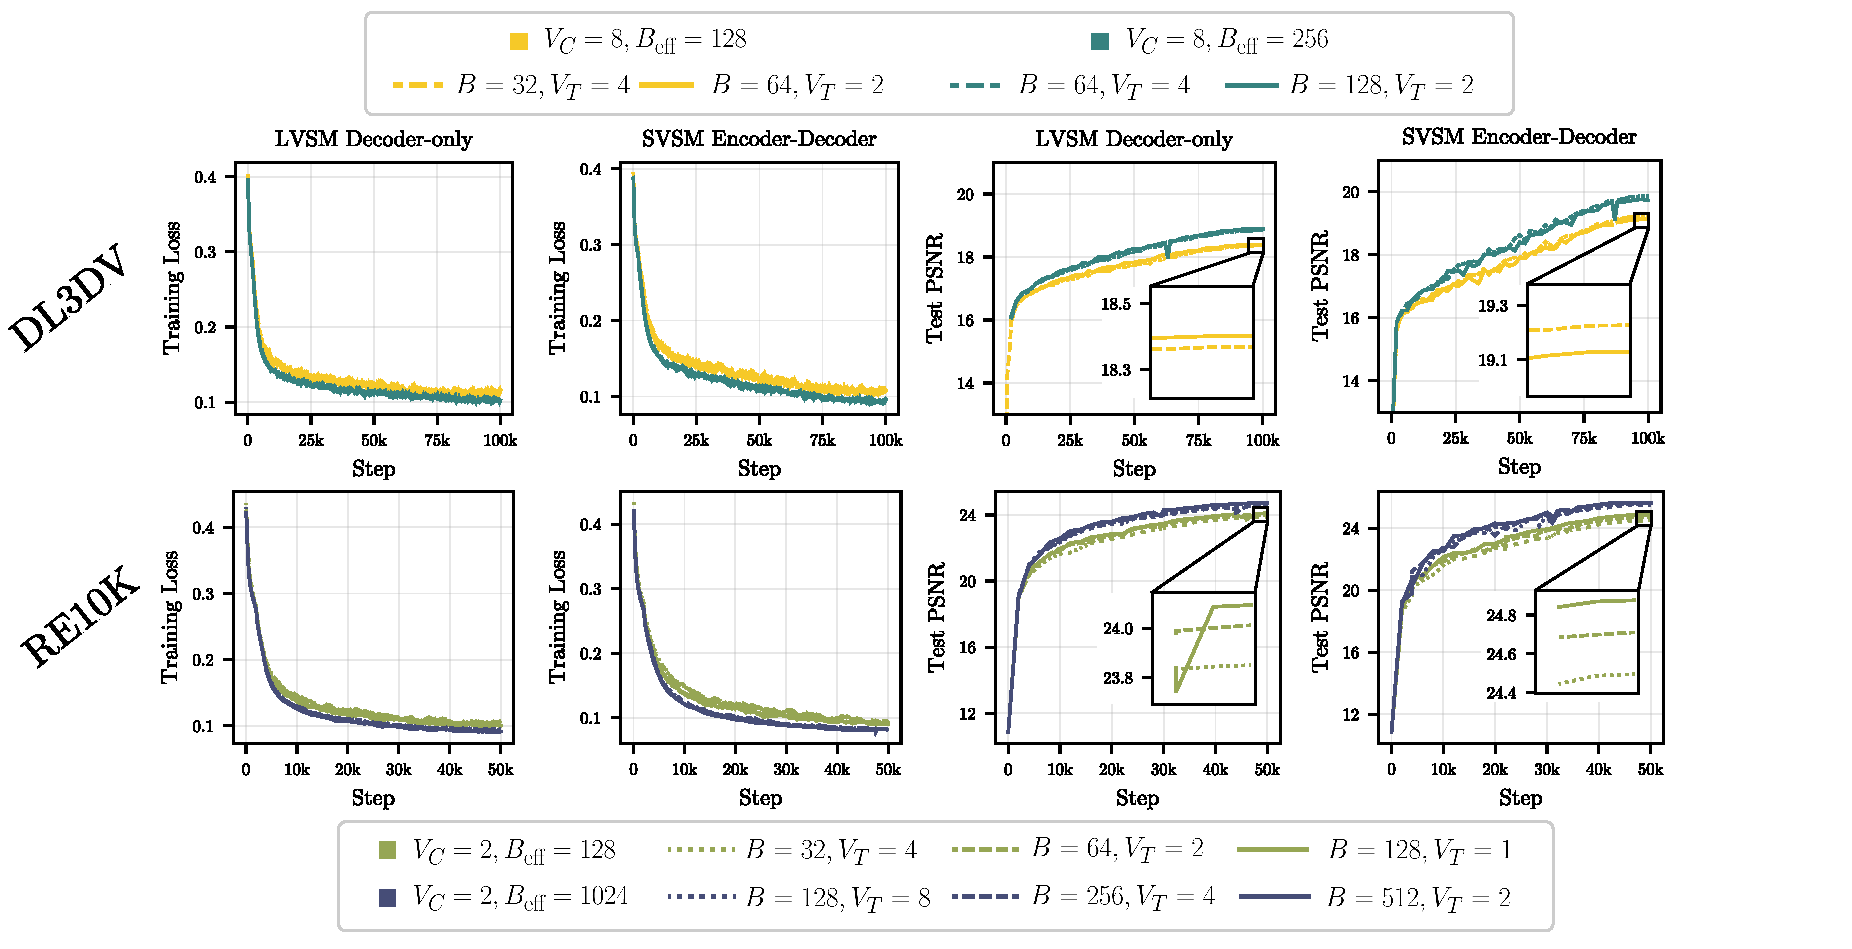
\includegraphics[width=\textwidth]{images/effective_batch_all.pdf}
    %
    \vspace{-0.8cm}
    \caption{\textbf{Effective Batch Size}. Training loss (smoothed with a rolling-average) and test PSNR measured throughout training across various paired $B$ and $V_T$ runs provide evidence for our effective batch size hypothesis: Models trained with the same product of number of scenes in the batch $B$ and number of reconstruction target views $V_T$, \emph{i.e.} runs with the same \emph{effective batch size} $B_{\text{eff}}$, perform the same and are colored identically. On $V_C = 8$ \textbf{(top)}, we sweep across $B_{\text{eff}} = $ \textcolor{B128first}{128}, \textcolor{B256}{256} on DL3DV, and on $V_C = 2$ \textbf{(bottom)}, we sweep across $B_{\text{eff}} =$ \textcolor{B128second}{128}, \textcolor{B1024}{1024} on RealEstate10K.
    \vspace{-1\baselineskip}
} % Main caption
    \label{fig:effective-batch} % Main label
\end{figure*}